\documentclass[a4paper,german,12pt,smallheadings]{scrartcl}
\usepackage[T1]{fontenc}
\usepackage[utf8]{inputenc}
\usepackage{babel}
\usepackage{geometry}
\usepackage{pdfpages}
\usepackage{tikz}
\usetikzlibrary{calc,intersections,fadings}
\usepackage{wrapfig}
\usepackage[fleqn]{amsmath}
\usepackage{amssymb}
\usepackage{float}
\usepackage{enumerate}
\usepackage{listings} % Source code
\usepackage{lscape} % landscape
\usepackage{commath} % http://tex.stackexchange.com/questions/14821/whats-the-proper-way-to-typeset-a-differential-operator
\usepackage{cancel}
\usepackage[fleqn]{mathtools}
\usepackage{xcolor}
\usepackage{pstricks}
\usepackage{pst-plot}
\usepackage{pst-math}
\usepackage{pst-pdf}
\usepackage{pstricks-add}
\usepackage[numbers]{natbib}
\usepackage{url}
% Number only referenced equations
%\mathtoolsset{showonlyrefs}

%\usepackage{wrapfig}
\usepackage{siunitx}
\sisetup{separate-uncertainty=true,locale=DE}

% http://tex.stackexchange.com/questions/38818/best-way-to-denote-an-angle-in-tikz
\newcommand\markangle[6][red]{% [color] {X} {origin} {Y} {mark} {radius}
  % filled circle: red by default
  \begin{scope}
    \path[clip] (#2) -- (#3) -- (#4);
    \fill[color=#1,fill opacity=0.5,draw=#1,name path=circle]
    (#3) circle (#6mm);
  \end{scope}
  % middle calculation
  \path[name path=line one] (#3) -- (#2);
  \path[name path=line two] (#3) -- (#4);
  \path[%
  name intersections={of=line one and circle, by={inter one}},
  name intersections={of=line two and circle, by={inter two}}
  ] (inter one) -- (inter two) coordinate[pos=.5] (middle);
  % bissectrice definition
  \path[%
  name path=bissectrice
  ] (#3) -- (barycentric cs:#3=-1,middle=1.2);
  % put mark
  \path[
  name intersections={of=bissectrice and circle, by={middleArc}}
  ] (#3) -- (middleArc) node[pos=1.3] {#5};
  }

% New command for color underlining
\usepackage{xcolor}
\newcommand\invisiblesection[1]{%
    \refstepcounter{section}%
      \addcontentsline{toc}{section}{\protect\numberline{\thesection}#1}%
        \sectionmark{#1}}
\newsavebox\MBox
\newcommand\colul[2][red]{{\sbox\MBox{$#2$}%
  \rlap{\usebox\MBox}\color{#1}\rule[-1.2\dp\MBox]{\wd\MBox}{0.5pt}}}

\restylefloat{table}
\geometry{a4paper, top=15mm, left=20mm, right=10mm, bottom=20mm, headsep=10mm, footskip=12mm}
\linespread{1.5}
\setlength\parindent{0pt}
\DeclareMathOperator{\Tr}{Tr}
\DeclareMathOperator{\Var}{Var}
\begin{document}
\bibliographystyle{unsrt}

\begin{titlepage}
\newcommand{\HRule}{\rule{\linewidth}{0.5mm}}

\begin{center}
  \textsc{\Large Physikalisches Grundpraktkum 1}
  \HRule\\[0.4 cm]
  {\huge \bfseries Gleichmäßig beschleunigte Drehbewegungen}
  \HRule\\[0.4 cm]

  \begin{minipage}{0.65\textwidth}
  \begin{flushleft}
    Markus Fenske \texttt{<iblue@zedat.fu-berlin.de>} \\
    Paul Rahmann \texttt{<paulrahmann@zedat.fu-berlin.de>}
  \end{flushleft}
  \end{minipage}
  \hfill
  \begin{minipage}{0.30\textwidth}
  \begin{flushright}
    Tutor: Christian Hindermann \\
    Versuchstag: 6. Juni 2014
  \end{flushright}
  \end{minipage}

  \vspace{1cm}

  \tableofcontents


  %{\large \today}
  \vfill
\end{center}
\newpage

\end{titlepage}

\allowdisplaybreaks % Seitenumbrüche in Formeln erlauben

\section{Physikalische Grundlagen}
\subsection{Tunneleffekt}

\begin{figure}[h!]
  \centering
  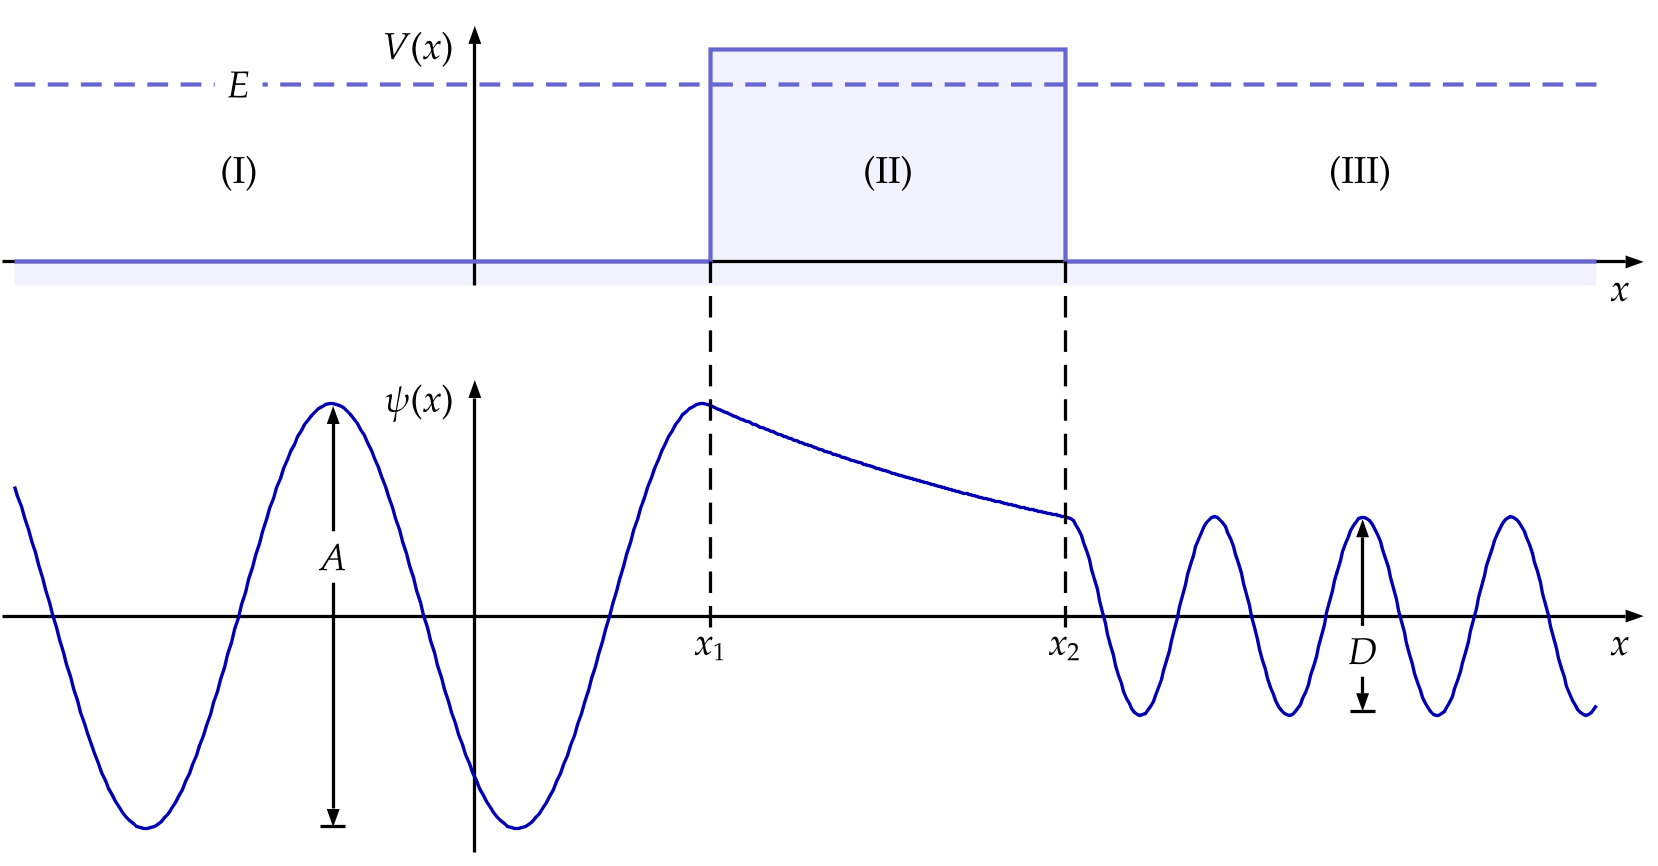
\includegraphics[width=1.0 \textwidth]{pic2.png}
  \caption{Lösung der Schrödingergleichung an einer Potentialstufe.\citep{pic2}}
\end{figure}

Gegeben sei ein Teilchen und eine Potentialstufe. Ist diese Potentialstufe
größer als die kinetische Energie des Teilchens, ist es dem Teilchen in
klassischer Betrachtung unmöglich, diese zu überwinden. In einer
quantenmechanischen Betrachtung gilt dies nicht mehr. Das Teilchen kann den
Potentialberg durchqueren. Man spricht veranschaulichend vom ``Tunneleffekt''.
Dieser ergibt sich direkt aus der Lösung der stationären eindimensionalen
Schrödingergleichung.

\begin{equation}
  \del{V - \frac{\hbar^2}{2m} \frac{\partial^2}{\partial x^2}} \Psi(x) = E \Psi(x)
\end{equation}

Wir betrachten ein kastenförmiges Potential.

\begin{equation}
  V(x) = \begin{cases} V_0 & \text{falls } x_1 \le x \le x_2 \\ 0 & \text{sonst} \end{cases}
\end{equation}

Wenn das Teilchen nun von $-\infty$ einläuft, erhalten wir drei verschiedene
stetig aneinander anschließende Lösungen

\begin{align*}
  \Psi_{I}(x) &= A e^{ikx} + B e^{-ikx} \\
  \Psi_{II}(x) &= C e^{\kappa x} + D e^{-\kappa x} \\
  \Psi_{III} &= F e^{ikx}
\end{align*}

mit den Koeffizienten

\begin{align*}
  k &= \sqrt{\frac{2mE}{\hbar^2}} \\
  \kappa &= \sqrt{\frac{2m (V_0 - E)}{\hbar^2}}
\end{align*}

Diese Modell lässt sich leider nur qualitativ auf das Rastertunnelmikroskop
übertragen. Beim Rastertunnelmikroskop wird eine Spitze im Abstand von wenigen
Angström über eine Probe gefahren. Zwischen Probe und Spitze wird eine Spannung
angelegt, das Potential ist somit in erster Näherung linear abfallend. Auch ist
das Problem nicht mehr als eindimensional zu betrachten. Um den Tunnelstrom
theoretisch vorherzusagen sind umfangreichere Betrachtungen nötig, so dass wir
hier nur das Ergebnis von \citep{hpa1982} wiedergeben wollen.

\begin{equation}
  I_{T} \propto \frac{V_T}{s} \exp \del{-A \phi^{1/2} s}
\end{equation}

Dabei ist $V_T$ die Tunnelspannung, $s$ der Abstand zwischen Probe und Spitze,
$A$ eine vom Zwischenraum abhängige Konstante und $\phi$ die Austrittsarbeit
aus der Probe an der gegebenen Stelle. Im Vakuum gilt
$A \approx 1{,}02 \AA^{-1} \text{eV}^{-1/2}$ nach \citep{versuchsanleitung}

\subsection{Piezoelektrischer Effekt}

Bestimmte Kristalle erzeugen bei Streckung oder Stauchung eine elektrische
Spannung. Dies ist dadurch erklärbar, dass sich durch die Verformung die
Schwerpunkte der positiven und negativen Ladungen verschieben. In den
Elementarzellen entstehen somit Dipole, die sich zu eine makroskopisch
messbaren Spannung aufsummieren. Umgekehrt entstecht durch Anlegen einer
Spannung eine Verformung. Dies wird im Rastertunnelmikroskop benutzt, um die
Spitze in sehr genauen Bereichen zu bewegen (rastern)\citep{versuchsanleitung}.

\subsection{Regelkreis}

Um den Tunnelstrom konstant zu halten, wird die Spitze der Probe bei einer
X-Y-Lageveränderung durch einen Regelkreis nachgeführt. Dazu wird der
tatsächliche Wert mit dem Sollwert verglichen und die Spitze entsprechend
bewegt.

\subsection{Tunnelspektroskopie}

Aus der X-Y-Spannung und der Z-Spannung erhält man durch zurückrechnen den
dreidimensiolen Ort der Spitze. Diese fährt die Äquipotentialflächen der
elektronischen Struktur der Probe ab, was Rückschlüsse auf die Probe erlaubt
(Tunnelspektroskopie).

\subsection{Räumliche Struktur von Festkörpern}

Festkörper im physikalischen bestehen aus sich periodisch wiederholenden
Strukturen. Das Modell geht dabei von einem unendlichen Kristall aus, der
translationssymmetrisch ist. Verschiebt man ihn um einen Gittervektor, erhält
man den Ausgangskristall. Festkörper lassen sich dabei gemäß ihrer
Gittervektoren in verschiedene Kristallsysteme einordnen.

Beim untersuchten Graphit handelt es sich um Lagen aus hexagonalen Kristallen.

\begin{figure}[h!]
  \centering
  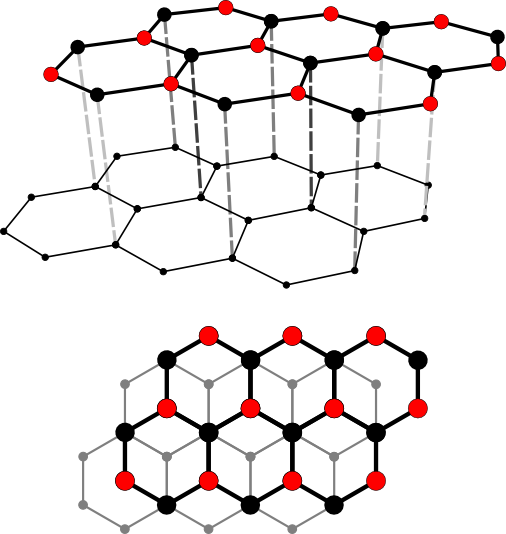
\includegraphics[width=0.6 \textwidth]{pic3.png}
  \caption{Grafitschichten in zwei verschiedenen Ansichten.\citep{pic3}}
\end{figure}

\subsection{Fouriertransformation}

Zur Analyse periodischer Strukturen ist die diskrete Fouriertransformation
geeignet. Dabei wird ein Datensatz $(a_0, a_1, \dots, a_{N-1})$ aus dem Ortsraum in
den Frequenzraum transformiert.

\begin{equation}
  \hat{a}_k = \sum_{j=0}^{N-1} \exp\del{2 \pi \text{i} \frac{jk}{N}} a_j
\end{equation}

Transformiert man das Signal so, erhält man die Frequenzkomponenten. Im
zweidimensionalen ist dies geeignet, um die reziproken Gittervektoren zu
erhalten.


\addcontentsline{toc}{section}{Literatur}
\bibliography{literatur}

\end{document}
